\section*{Singular Homology with Coefficients}

Aim of this section is to construct for each $n \in \omega$ a functor $H_n : \mathsf{Top} \to \mathsf{AbGrp}$, called the \textit{$n$-th singular homology functor}.

\subsection*{Simplices and Affinely Linear Mappings}

\begin{definition}[Affinely Independent]
	Let $n,k \in \omega$. A family $(v_0,\dots,v_k)$ in $\mathbb{R}^n$ is said to be \bld{affinely independent}, iff the following condition is satisfied: Given $\lambda_0,\dots,\lambda_k \in \mathbb{R}$ such that
	\begin{equation*}
		\sum_{i = 0}^k \lambda_i = 0 \qquad \text{and} \qquad \sum_{i = 0}^k \lambda_i v_i = 0
	\end{equation*}
	\noindent implies $c_0 = \dots = c_k = 0$.
\end{definition}

\begin{lemma}
	\label{lem:affinely_independent}
	Let $n,k \in \omega$. Then a family $(v_0,\dots,v_k)$ in $\mathbb{R}^n$ is affinely independent if and only if $(v_1 - v_0,\dots,v_k - v_0)$ is linearly independent in $\mathbb{R}^n$.
\end{lemma}

\begin{exercise}
	\label{ex:affinely_independent}
	Prove lemma \ref{lem:affinely_independent}.
\end{exercise}

\begin{definition}[Simplex]
	\label{def:simplex}
	Let $n,k \in \omega$ and $(v_0,\dots,v_k)$ affinely independent in $\mathbb{R}^n$. Define the \bld{simplex spanned by $(v_0,\dots,v_k)$}, written $[v_0,\dots,v_n]$, to be the topological subspace 
	\begin{equation*}
		[v_0,\dots,v_k] := \cbr[4]{\sum_{i = 0}^k \lambda_i v_i : \lambda_i \in \mathbb{R}_{\geq 0} \> \text{and} \> \sum_{i = 0}^k \lambda_i = 1} \subseteq \mathbb{R}^n.
	\end{equation*}
	Moreover, each of the $v_i$'s, $i = 0,\dots,k$, is called a \bld{vertex} of the simplex $[v_0,\dots,v_k]$.
\end{definition}

\begin{remark}
	Let $\sigma := [v_0,\dots,v_k]$ be a simplex spanned by $(v_0,\dots,v_k)$. Then we will also simply call $\sigma$ a $k$-simplex in $\mathbb{R}^n$.
\end{remark}

\begin{example}[Standard Simplex]
	Let $n \in \omega$. Then the family $(e_0,\dots,e_n)$ in $\mathbb{R}^n$, where $e_0 := 0$ and $(e_1,\dots,e_n)$ is the standard oriented basis of $\mathbb{R}^n$, is affinely independent by exercise \ref{ex:affinely_independent}. The $n$-simplex spanned by this family is called the \bld{standard $n$-simplex} and is denoted by $\Delta^n$.
	\begin{figure}[h!tb]
		\centering
		\begin{subfigure}[b]{.3\textwidth}
			\centering
			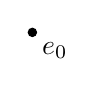
\begin{tikzpicture}[scale = 3]
				\draw[fill] (0,1) circle [radius=.5pt] node[below right]{$e_0$};
			\end{tikzpicture}
			\caption{$\Delta^0$.}
			\label{fig:Delta^0}
		\end{subfigure}
		~
		\begin{subfigure}[b]{.3\textwidth}
			\centering
			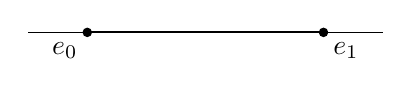
\begin{tikzpicture}[scale = 3]
    			% Draw axes
				\draw (-.75,1) -- (.75,1);
				\draw [thick] (-.5,1) -- (.5,1);
				\draw[fill] (-.5,1) circle [radius=.5pt] node[below left]{$e_0$};
				\draw[fill] (.5,1) circle [radius=.5pt] node[below right]{$e_1$};
			\end{tikzpicture}
			\caption{$\Delta^1$.}
			\label{fig:Delta^1}
		\end{subfigure}
		~
		\begin{subfigure}[b]{.3\textwidth}
			\centering
			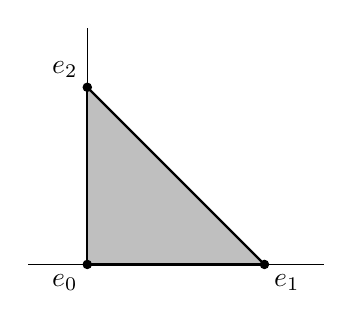
\begin{tikzpicture}[scale = 3]
    			% Draw axes
				\draw (-.25,1) -- (1,1);
				\draw (0,1) -- (0,2);
				\fill[fill=gray!50] (0,1)--(.75,1)--(0,1.75);
				\draw [thick] (0,1) -- (.75,1);
				\draw [thick] (0,1) -- (0,1.75);
				\draw [thick] (.75,1) -- (0,1.75);
				\draw[fill] (0,1) circle [radius=.5pt] node[below left]{$e_0$};
				\draw[fill] (.75,1) circle [radius=.5pt] node[below right]{$e_1$};
				\draw[fill] (0,1.75) circle [radius=.5pt] node[above left]{$e_2$};
			\end{tikzpicture}
			\caption{$\Delta^2$.}
			\label{fig:Delta^2}
		\end{subfigure}
		\caption{Standard $n$-simplices.}
	\end{figure}
\end{example}

\begin{lemma}
	\label{lem:barycentric_coordinates}
	Let $n,k \in \omega$ and $[v_0,\dots,v_k]$ a $k$-simplex in $V$. Then any $x \in [v_0,\dots,v_k]$ admits a unique representation $x = \sum_{i = 0}^k \lambda_i v_i$.
\end{lemma}

\begin{exercise}
	Prove lemma \ref{lem:barycentric_coordinates}.
\end{exercise}

\begin{definition}[Affinely Linear Mapping]
	Let $n,m in \omega$. A mapping $A : \mathbb{R}^n \to \mathbb{R}^m$ is said to be \bld{affinely linear}, iff there exists an $\mathbb{R}$-linear vector space morphism $L : \mathbb{R}^n \to \mathbb{R}^m$ and $y \in \mathbb{R}^m$, such that 
	\begin{equation*}
		A(x) = L(x) + y
	\end{equation*}
	\noindent holds for all $x \in \mathbb{R}^n$.
\end{definition}

\begin{exercise}
	\label{ex:affinely_linear}
	Show that the composition of affinely linear mappings is again affinely linear.
\end{exercise}

\begin{proposition}[Affine Map induced by Vertex Map]
	\label{prop:affine_map_induced_by_vertex_map}
	Let $n,k,m \in \omega$ and $\sigma := [v_0,\dots,v_n]$ a $k$-simplex in $\mathbb{R}^n$. Given a function $f : \cbr{v_0,\dots,v_k} \to \mathbb{R}^m$, there exists a unique extension $\wtilde{f} : \sigma \to \mathbb{R}^m$, which is the restriction of an affinely linear map.
\end{proposition}

\begin{proof}
	We show first existence and then uniqueness.
	\begin{enumerate}[label = \textit{Step \arabic*:},wide=0pt]
		\item \textit{Existence.} By exercise \ref{ex:affinely_independent}, $(v_1 - v_0,\dots, v_k - v_0)$ is linearly independent in $\mathbb{R}^n$. Since $\mathbb{R}^n$ is finite dimensional, we may complete this linearly independent subset to a basis of $\mathbb{R}^n$. Hence there exists a unique vector space morphism $L : \mathbb{R}^n \to \mathbb{R}^m$, mapping 
			\begin{equation*}
				v_i - v_0 \mapsto f(v_i) - f(v_0),
			\end{equation*}
			\noindent for $i = 1,\dots,k$ and to the zero vector else. Now $A : \mathbb{R}^n \to \mathbb{R}^m$ defined by
			\begin{equation*}
				 A := L - L(v_0) + f(v_0)
			\end{equation*}
			\noindent is the map we are looking for.
		\item \textit{Uniqueness.} Given another such extension $\wtilde{g} : \sigma \to \mathbb{R}^m$ of $f$, say $\wtilde{g} = \wtilde{L} + y$, we have that $\wtilde{L}(v_i) = f(v_i) - y$ for all $i = 0,\dots,k$. Thus we compute 
			\begin{equation*}
				\wtilde{g}\del[4]{\sum_{i = 0}^k \lambda_i v_i} = \sum_{i = 0}^k \lambda_i \wtilde{L}(v_i) + y = \sum_{i = 0}^k \lambda_i f(v_i) - \sum_{i = 0}^k \lambda_i y + y = \sum_{i = 0}^k \lambda_i f(v_i).
			\end{equation*}
	\end{enumerate}
\end{proof}


\subsection*{Free Abelian Groups}

\begin{proposition}
	\label{prop:F_set_abgrp}
	The forgetful functor $U : \mathsf{AbGrp} \to \mathsf{Set}$ admits a left adjoint.	
\end{proposition}

\begin{proof}
	We have to construct a functor $F : \mathsf{Set} \to \mathsf{AbGrp}$. Let $S$ be a set. Define 
	\begin{equation*}
		F(S) := \cbr[1]{f \in \mathbb{Z}^S : \supp f \text{ is finite}}.
	\end{equation*}
	Equipped with pointwise addition, $F(S)$ is an abelian group. There is a natural inclusion $\iota : S \hookrightarrow U\del[1]{F(S)}$ sending $x \in S$ to the function taking the value one at $x$ and zero else. Hence we may regard elements of $F(S)$ as formal linear combinations $\sum_{x \in S}m_x x$, where $m_x \in \mathbb{Z}$ for all $x \in S$. On morphisms $f : S \to T$ in $\mathsf{Set}$, define $F(f) : F(S) \to F(T)$ simply by setting $F(f)\del[1]{\sum_{x \in S}m_x x} := \sum_{x \in S}m_x f(x)$.\\	
	Let $G \in \ob(\mathsf{AbGrp})$ be an abelian group and $\varphi \in \mathsf{AbGrp}\del[1]{F(S), G}$ a morphism of groups. Define $\wbar{\varphi} \in \mathsf{Set}\del[1]{S,U(G)}$ by $\wbar{\varphi} := U(\varphi)$. Conversly, if we have $f \in \mathsf{Set}\del[1]{S,U(G)}$, define $\wbar{f} \in \mathsf{AbGrp}\del[1]{F(S),G}$ by $\wbar{f}\del[1]{\sum_{x \in S} m_x x} := \sum_{x \in S} m_x f(x)$. This is well defined since all but finitely many $m_x$ are zero and $G$ is abelian. It is easy to check that $\wbar{f}$ is indeed a morphism of groups. Let $\varphi \in \mathsf{AbGrp}\del[1]{F(S),G}$. Then
	\begin{align*}
		\wbar{\wbar{\varphi}}\del[4]{\sum_{x \in S} m_x x} &= \sum_{x \in S}m_x \wbar{\varphi}(x)\\
		&= \sum_{x \in S} m_x U(\varphi)(x)\\
		&= \sum_{x \in S} m_x \varphi(x)\\
		&= \varphi \del[4]{\sum_{x \in S} m_x x}.
	\end{align*}
	And for $f \in \mathsf{Set}\del[1]{S,U(G)}$ we have that
	\begin{equation*}
		\wbar{\wbar{f}}(x) = U(\wbar{f})(x) = \wbar{f}(x) = f(x). 
	\end{equation*}
	\noindent Hence $\wbar{\wbar{\varphi}} = \varphi$ and $\wbar{\wbar{f}} = f$ and so we have a bijection
	\begin{equation*}
		\mathsf{AbGrp}\del[1]{F(S),G} \cong \mathsf{Set}\del[1]{S,U(G)}.
	\end{equation*}
	The mapping $f \mapsto \wbar{f}$ will be referred to as \bld{extending by linearity}. To check naturality in $S$ and $G$ is left as an exercise.
\end{proof}

\begin{exercise}
	In proposition \ref{prop:F_set_abgrp}, check that $F : \mathsf{Set} \to \mathsf{AbGrp}$ is indeed a functor, called the \bld{free functor from $\mathsf{Set}$ to $\mathsf{AbGrp}$}, and the naturality of the bijection in both arguments. 
\end{exercise}

\begin{definition}[Free Abelian Group]
	Let $F : \mathsf{Set} \to \mathsf{AbGrp}$ be the free functor. For any set $S$, we call $F(S)$ the \bld{free group generated by $S$}.
\end{definition}


\begin{theorem}
	There is a functor $\mathsf{Top} \to \mathsf{Comp}$.
	\label{thm:singular_complex}
\end{theorem}

\begin{proof}
	The proof is divided into several steps. Let us denote $C_\bullet : \mathsf{Top} \to \mathsf{Comp}$ for the claimed functor.
	\begin{enumerate}[label = \textit{Step \arabic*:},wide = 0pt, itemsep = 1.5ex]
		\item \textit{Construction of a sequence of abelian groups.} Let $v_0,\dots,v_k \in \mathbb{R}^n$ for some $n,k \in \omega$. We say that $(v_0,\dots,v_k)$ is \bld{affinely independent} if $(v_1 - v_0,\dots, v_k - v_0)$ is linearly independent. We define the \bld{k-simplex spanned by $(v_0,\dots,v_k)$}, written $\sbr[0]{v_0,\dots,v_k}$, to be
			\begin{equation}
				\textstyle{\sbr[0]{v_0,\dots,v_k} := \cbr[1]{\sum_{i = 0}^k s_i v_i : s_i \geq 0 \text{ for all } i = 0,\dots,k \text{ and } \sum_{i = 0}^k s_i = 1}}.
			\end{equation}
			\noindent equipped with the subspace topology. Moreover, we define the \bld{standard $n$-simplex $\Delta^n$} to be the $n$-simplex spanned by $(e_0,\dots,e_n)$ where $e_0 := 0 \in \mathbb{R}^n$ and $(e_1,\dots,e_n)$ is the standard ordered basis of $\mathbb{R}^n$. Let $X \in \ob(\mathsf{Top})$. Define a \bld{singular $n$-simplex in $X$} to be a morphism $\sigma \in \mathsf{Top}(\Delta^n,X)$. Let $n \in \mathbb{Z}$. Define
			\begin{equation}
				C_n(X) := \ccases{F\del[1]{\mathsf{Top}(\Delta^n,X)} & n \geq 0,\\
									0 & n < 0.}
			\end{equation}
			We will call elements of $C_n(X)$ \bld{singular $n$-chains}.
		\item \textit{Construction of boundary operators.} Let $X \in \ob(\mathsf{Top})$ and $\sigma$ a singular $n$-simplex in $X$ for $n \geq 1$. We define $\varphi^n_k : \Delta^{n-1} \to \Delta^n$, called the \bld{$k$-th face map}, to be the unique affine map determined by the vertex map
			\begin{equation*}
				\begin{matrix}
					& \varphi_k^n\\
					e_0 & \mapsto & e_0\\
					\vdots & & \vdots\\
					e_{k - 1} & \mapsto & e_{k - 1}\\
					e_k & \mapsto & e_{k + 1}\\
					\vdots & & \vdots\\
					e_{n - 1} & \mapsto & e_n.
				\end{matrix}
			\end{equation*}
			Explicitely, given $\sum_{i = 0}^{n - 1} s_i e_i \in \Delta^{n - 1}$, we have that (see \cite[152]{lee:topological_manifolds:2011})
			\begin{equation*}
				\varphi_k^n \del[4]{\sum_{i = 0}^{n - 1}s_i e_i} = \sum_{i = 0}^{n - 1}s_i \varphi_k^n(e_i).
			\end{equation*}
			Define now
			\begin{equation}
				\partial \sigma := \sum_{k = 0}^n (-1)^k \sigma \circ \varphi_k^n \in U\del[1]{C_{n - 1}(X)} 
			\end{equation}
			\noindent to be the \bld{boundary of $\sigma$}. Moreover, the \bld{singular boundary operator} is defined to be $\wbar{\partial_n}$ and $\partial_n := 0$ for $n \leq 0$.
		\item \textit{$\partial_n \circ \partial_{n + 1} = 0$ for all $n \in \mathbb{Z}$.} It is enough to consider $n \geq 1$, since $\partial_n \circ \partial_{n + 1} = 0$ holds trivially in the other cases. Let $X \in \ob(\mathsf{Top})$ and $\sigma \in \mathsf{Top}(\Delta^{n+1},X)$. Then we have
			\begin{align*}
				(\partial_n \circ \partial_{n + 1})(\sigma) &= \partial_n \del[4]{\sum_{k = 0}^{n + 1} (-1)^k \sigma \circ \varphi^{n + 1}_k}\\
				&= \sum_{k = 0}^{n + 1} (-1)^k \partial_n\del[1]{\sigma \circ \varphi^{n + 1}_k}\\
				&= \sum_{k = 0}^{n + 1}\sum_{j = 0}^n (-1)^{k + j} \sigma \circ \varphi^{n + 1}_k \circ \varphi^n_j\\
				&= \sum_{0 \leq k \leq j \leq n}(-1)^{k + j} \sigma \circ \varphi^{n + 1}_k \circ \varphi^n_j + \sum_{0 \leq j < k \leq n + 1}(-1)^{k + j} \sigma \circ \varphi^{n + 1}_k \circ \varphi^n_j\\
				&= \sum_{0 \leq j \leq k \leq n}(-1)^{k + j} \sigma \circ \varphi^{n + 1}_j \circ \varphi^n_k + \sum_{0 \leq j <k \leq n + 1}(-1)^{k + j} \sigma \circ \varphi^{n + 1}_k \circ \varphi^n_j\\
				&= \sum_{0 \leq j < k \leq n + 1}\del[1]{(-1)^{k + j - 1} \sigma \circ \varphi^{n + 1}_j \circ \varphi^n_{k - 1} + (-1)^{k + j} \sigma \circ \varphi^{n + 1}_k \circ \varphi^n_j}
			\end{align*}
			Since $\varphi_j^{n + 1} \circ \varphi_{k - 1}^n = \varphi_k^{n + 1} \circ \varphi_j^n$, it follows that
			\begin{equation*}
				\partial_n \circ \partial_{n + 1} = 0.
			\end{equation*}
			Indeed, consider the following chart of vertex maps:
			\begin{equation*}
				\begin{matrix}
					& \varphi_{k - 1}^n & & \varphi_j^{n + 1}\\
					e_0 & \mapsto & e_0 & \mapsto & e_0\\
					\vdots & & \vdots & & \vdots\\
					e_{j - 1} & \mapsto & e_{j - 1} & \mapsto & e_{j - 1}\\
					e_j & \mapsto & e_j & \mapsto & e_{j + 1}\\
					\vdots & & \vdots\\
					e_{k - 1} & \mapsto & e_{k - 1} & \mapsto & e_{k + 1}\\
					e_k & \mapsto & e_{k + 1} & \mapsto & e_{k + 2}\\
					\vdots & & \vdots\\
					e_{n - 1} & \mapsto & e_n & \mapsto & e_{n + 1}
				\end{matrix}
				\qquad\qquad\qquad
				\begin{matrix}
					& \varphi_j^n & & \varphi_k^{n + 1}\\
					e_0 & \mapsto & e_0 & \mapsto & e_0\\
					\vdots & & \vdots & & \vdots\\
					e_{j - 1} & \mapsto & e_{j - 1} & \mapsto & e_{j - 1}\\
					e_j & \mapsto & e_{j + 1} & \mapsto & e_{j + 1}\\
					\vdots & & \vdots\\
					e_{k - 1} & \mapsto & e_k & \mapsto & e_{k + 1}\\
					e_k & \mapsto & e_{k + 1} & \mapsto & e_{k + 2}\\
					\vdots & & \vdots\\
					e_{n - 1} & \mapsto & e_n & \mapsto & e_{n + 1}
				\end{matrix}.
			\end{equation*}
		\item \textit{Construction of chain maps.} Let $X,Y \in \ob(\mathsf{Top})$ and $f \in \mathsf{Top}(X,Y)$. For $n \geq 0$, define $f_n^\# : \mathsf{Top}(\Delta^n,X) \to U\del[1]{C_n(Y)}$ by $f^\# := f \circ \sigma$. Extending this map by linearity yields a homomorphism $f_n^\# : C_n(X) \to C_n(Y)$. Moreover, set $f_n^\# := 0$ for $n < 0$. Let $n \geq 1$ and $\sigma \in \mathsf{Top}(\Delta^n,X)$. Then on one hand we have
			\begin{equation*}
				(f_{n - 1}^\# \circ \partial_n)(\sigma) = f^\#_{n - 1}\del[4]{\sum_{k = 0}^n (-1)^k \sigma \circ \varphi^n_k} = \sum_{k = 0}^n (-1)^k f \circ \sigma \circ \varphi^n_k
			\end{equation*}
			\noindent and on the other
			\begin{equation*}
				(\partial_n \circ f^\#_n)(\sigma) = \partial_n(f \circ \sigma) = \sum_{k = 0}^n (-1)^k f \circ \sigma \circ \varphi^n_k.
			\end{equation*}
	\end{enumerate}
	Checking, that $C_\bullet$ is indeed a functor is left as an exercise.
\end{proof}

\begin{exercise}
	Show that $C_\bullet : \mathsf{Top} \to \mathsf{Comp}$ is a functor.
\end{exercise}

\subsection*{The Homology Functor}
\begin{definition}[Singular Homology Functor]
	Let $n \in \mathbb{Z}$. The composition 
	\begin{equation}
		H_n \circ C_\bullet : \mathsf{Top} \to \mathsf{AbGrp}
	\end{equation}
	\noindent of the singular chain complex functor $C_\bullet$ in theorem \ref{thm:singular_complex} and the $n$-th homology functor of proposition \ref{prop:homology_functor} is called the \bld{$n$-th singular homology functor}, written $H^{\mathrm{sing}}_n$.
\end{definition}

\begin{remark}
	For notational purposes we will often refer to the functor $H_n^{\mathrm{sing}}$ simply as $H_n$.
\end{remark}

%%%%%%%%%%%%%%%%%%%%%%%%%%%%%%%%%%%%%%%%%%%%%%%%%%%%%%%%%%%%%%%%%%%%%%%%%%%%%%%%%%%%%%%%%%%%%%%%%%%%%%%%%%%%%
%Relative and Reduced Homology																				%
%%%%%%%%%%%%%%%%%%%%%%%%%%%%%%%%%%%%%%%%%%%%%%%%%%%%%%%%%%%%%%%%%%%%%%%%%%%%%%%%%%%%%%%%%%%%%%%%%%%%%%%%%%%%%
\subsection*{Relative Homology}

\begin{proposition}
	There is a functor $\mathsf{Top}^2 \to \mathsf{Comp}$.
\end{proposition}

\begin{proof}
	Let $(X,A) \in \ob(\mathsf{Top}^2)$. Then we have an inclusion $\iota : A \hookrightarrow X$. Moreover, we have that $C_n(\iota)$ is injective for all $n \in \mathbb{Z}$. Indeed, this is obvious for $n < 0$ and for $n \geq 0$, suppose that $\sum_k m_k \sigma_k \in \ker C_n(\iota)$, where the $\sigma_k$ are distinct. Then we have that $0 = C_n(\iota)\del[1]{\sum_k m_k \sigma_k} = \sum_k m_k \iota \circ \sigma_k$, where the $\iota \circ \sigma_k$ are also distinct. Thus we conclude $\sum_k m_k \sigma_k = 0$. Hence we can see $C_\bullet(A)$ as a subcomplex of $C_\bullet(X)$ and so we can define
	\begin{equation*}
		C_\bullet(X,A) := C_\bullet(X)/C_\bullet(A).
	\end{equation*}
	Moreover, on morphsisms $f \in \mathsf{Top}^2\del[1]{(X,A),(Y,B)}$ just let $C_\bullet(f)$ be the induced map.
\end{proof}

\begin{definition}[Relative Homology Functor]
	For $n \in \mathbb{Z}$, the functor 
	\begin{equation}
		H_n \circ C_\bullet : \mathsf{Top}^2 \to \mathsf{AbGrp}
	\end{equation}
	\noindent is called the \bld{$n$-th relative singular homology functor.}
\end{definition}
